\section{Persistent data management}
To save the data in form of events, tags and so on, an online database connection will be used. The database gives access to data quickly and from multiple locations. The problem with this solution is that it requires an internet connection. To work around this a strategy design pattern can be implemented to provide the application the possibility to store data locally if no connection is available and vice. versa. \\
The Data which must be persistant is the following objects:
\begin{itemize}
	\item Events
	\item Notifications - as long as they are not dismissed by the user
	\item Tags 
	\item User info - passwords, usernames and their connection.
\end{itemize}
To peek, post, update, delete LINQ can be used since it supports these features in a strong cross storage-platform language.\\\\

\newpage
\textbf{OO to RDBMS mapping:}

\begin{figure}[h!]
	\centering
		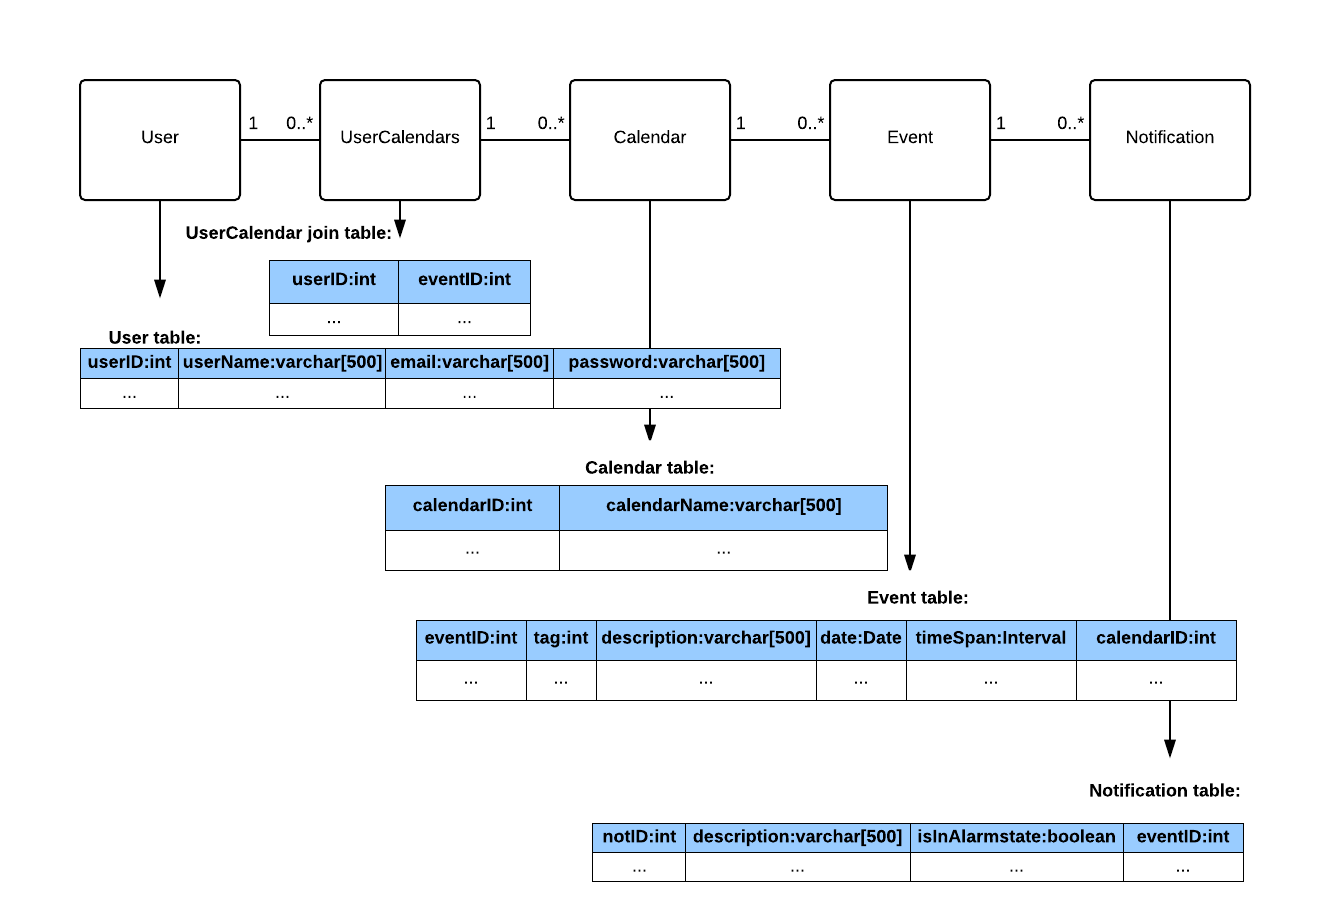
\includegraphics[scale=0.8]{OOtoRDBMSMapping}
	\caption{Zoom in to see details: Model of OO to RDBMS Mapping}
	\label{fig:OO to RDBMS Mapping}
\end{figure}

As for the primary, foreign and candidate keys it goes as following.\\
In the User table, the userID is the primary key. The candidate keys are userName and email, as these just as well could be the primary key as they always be unique.\\
In the Calendar table, the calendarID is the primary key.\\
In the Event table, the eventID is the primary key, while the calendarID is the foreign key.\\
In the Notification table,  the notID is the primary key, while the eventID is the foreign key.\\
Finally in the UserCalendars join table, both userID and eventID are foreign keys.\\